\documentclass{beamer}
\usetheme{metropolis}           % Use metropolis theme

\metroset{numbering=none}
\setmonofont{Fira Code}

\usepackage{minted}
\usemintedstyle{friendly}
\setminted{
    frame=none, %lines,
    framesep=2mm,
    baselinestretch=1.2,
    %bgcolor=lightgray,
    fontsize=\footnotesize,
    escapeinside=\#\#
    }
\usepackage{filecontents}

\usepackage{tikz}
\usetikzlibrary{fadings}
\usetikzlibrary{snakes}
\usetikzlibrary{positioning}
\usetikzlibrary{arrows}
\usetikzlibrary{shapes.symbols}

\usepackage{verbatimbox}

\definecolor{bg}{rgb}{0.85,0.85,0.85}

\setbeamertemplate{frametitle}
{
  \setbeamercolor{palette quaternary}{fg=orange}
  \setbeamercolor{titlelike}{parent=palette quaternary}
  \setbeamerfont{frametitle}{size=\Large,series=\bfseries}
  \insertframetitle
}

%\setbeamercolor{titlelike}{parent=palette primary,fg=orange}
%\setbeamercolor{frametitle}{bg=white!90!orange,fg=orange}
\setbeamercolor{frametitle}{bg=white, fg=orange}
\setbeamercolor{frametitle right}{bg=gray!60!white}
\setbeamertemplate{frametitle}[default][center]

\usebackgroundtemplate{%
  \tikz[overlay,remember picture]
     \tikzfading[name=fade out, inner color=transparent!90,
         outer color=transparent!75]
\node[at=(current page.center), scope fading=fade out] {
   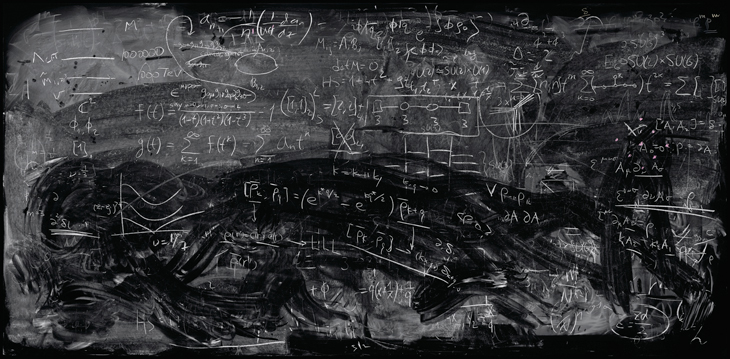
\includegraphics[height=\paperheight]{alejandro_guijarro_StanfordI}};
}

\title{Safe APIs from Ghosts of Departed Proofs}
\date{\today}
\author{Matt Noonan}
\institute{Kataskeue LLC \& Input Output HK}
\begin{document}

\begin{myverbbox}[\scriptsize]{\github}
git clone https://github.com/matt-noonan/gdp-talk
cd gdp-talk && stack ghci
\end{myverbbox}

\begin{frame}
\maketitle
\begin{tikzpicture}[overlay, remember picture]
  \node (A) [above left =2cm and 0.5cm of current page.south east] {\scriptsize{Play along at home!}};
  \node (B) [above =0.4cm of current page.south] {\github};
  \draw [thick, ->, >=stealth', in=90] (A.west) -> (B.north);
\end{tikzpicture}
\end{frame}

\usebackgroundtemplate{}

\begin{frame}{}
  \begin{quotation}
\noindent      [Rico Mariani] admonished us to think about
how we can build platforms that lead developers
to write great, high performance code such that
developers just fall into doing the “right thing”.
\medskip

\noindent
That concept really resonated with me. It is the
key point of good API design.
\bigskip

\noindent
\alert{We should build
APIs that steer and point developers in the right
direction.}\\
\phantom{x} \hfill — Brad Abrams
  \end{quotation}
  
\end{frame}

%%%%%%%%%%%%%%%%%%%%%%%%%%%%%%%%%%%%%%%%%%%%%%%%%%%%%%%%%%%%%%%%%%%%%%%%
  \section{How can we make good APIs?}   %%%%%%%%%%%%%%%%%%%%%%%%%%%%%%%%
%%%%%%%%%%%%%%%%%%%%%%%%%%%%%%%%%%%%%%%%%%%%%%%%%%%%%%%%%%%%%%%%%%%%%%%%

\begin{frame}{Narrowing the focus}
  Specifically, how can we make APIs that are:
  \begin{itemize}
    \bigskip
  \item {\alert{Safe.} \\ \qquad Incorrect use of the API should result in an error
    \\ \qquad at compile-time.}
    \bigskip
  \item {\alert{Ergonomic.} \\ \qquad Correct use of an API should not place an undue \\
    \qquad burden on the user.}
    \end{itemize}
\end{frame}


\begin{frame}{What is the goal?}
  In this talk, we will investigate how
  \bigskip\alert{
  \begin{itemize}
  \item{existentially-quantified type-level names for values,}
    \medskip
  \item{theorems as phantom types, and}
    \medskip
  \item{safe coercions}
  \end{itemize}}
  \bigskip
  
  \noindent can combine to provide a safe and ergonomic strategy for designing APIs
  with complex requirements.
\end{frame}

\begin{frame}{Unsafe idiom: explode}
  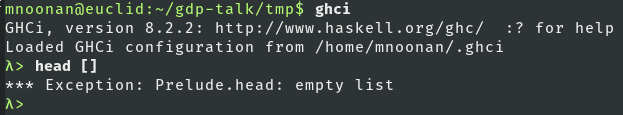
\includegraphics[width=0.8\paperwidth]{hsout}
\end{frame}

%% \begin{frame}{Unsafe strategy: explode?}
%%   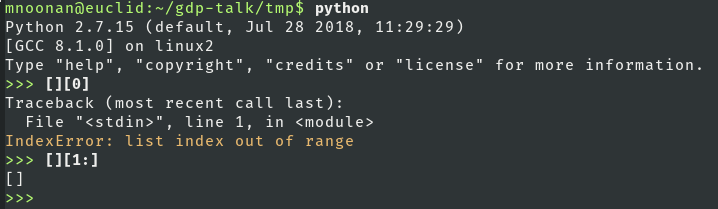
\includegraphics[width=0.8\paperwidth]{pyout}
%% \end{frame}

%% %%%%%%%%%%%%%%%%%%%%%%%%%%%%%%%%%%%%%%%%%%%%%%%%%%%%%%%%%%%%%%%%%%%%%%%%
%% \begin{frame}{Unergonomic strategy: special value}
%%   
\includegraphics[width=0.8\paperwidth]{lispout}
%% \end{frame}


%% %%%%%%%%%%%%%%%%%%%%%%%%%%%%%%%%%%%%%%%%%%%%%%%%%%%%%%%%%%%%%%%%%%%%%%%%

\begin{frame}{Unsafe idiom: anything goes}
   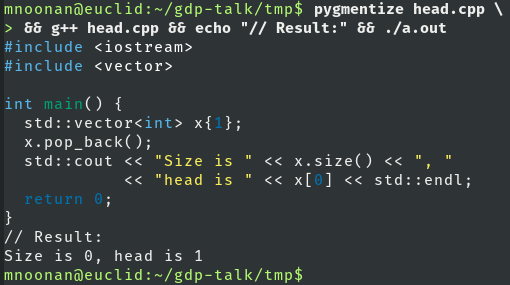
\includegraphics[width=0.8\paperwidth]{cppout}
\end{frame}

%%%%%%%%%%%%%%%%%%%%%%%%%%%%%%%%%%%%%%%%%%%%%%%%%%%%%%%%%%%%%%%%%%%%%%%%
\begin{filecontents*}{safehead.hs}
data NonEmptyList a = NonEmptyList a [a]
  
headNE :: NonEmptyList a -> a
headNE (NonEmptyList x xs) = x  
\end{filecontents*}
\begin{frame}{Safe idiom: use refinement types to restrict domain}
  \inputminted{haskell}{safehead.hs}
  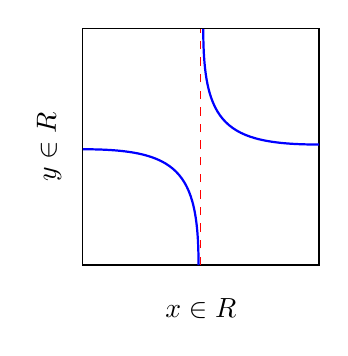
\begin{tikzpicture}[scale=0.3]
    \draw (0,0) -- (10,0) -- (10,10) -- (0,10) -- cycle;
    \draw[color=blue, thick] (0,4.9) .. controls (4,4.9) and (4.9,4) .. (4.9,0);
    \draw[color=blue, thick] (10,5.1) .. controls (6,5.1) and (5.1,6) .. (5.1,10);
    \draw[color=red, dashed] (5,0) -- (5,10);
    \node[anchor=south] at (5,-2.7) {$x \in \mathbb{R}$};
    \node[anchor=south, rotate=90] at (-0.5,5) {$y \in \mathbb{R}$};
  \end{tikzpicture}
  \hfill
  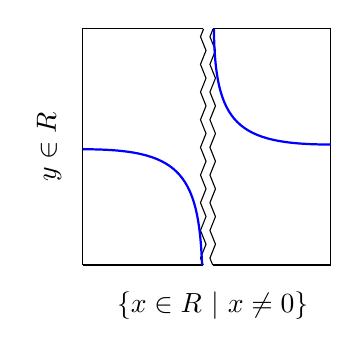
\begin{tikzpicture}[scale=0.3]
    \draw (0,0) -- (5.1,0);
    \draw[snake=zigzag, segment amplitude=1pt] (5.1,0) -- (5.1,10);
    \draw (5.1,10) -- (0,10) -- (0,0);
    \draw[color=blue, thick] (0,4.9) .. controls (4,4.9) and (4.9,4) .. (5.05,0);

    \draw (10.5,0) -- (5.5,0);
    \draw[snake=zigzag, segment amplitude=1pt] (5.5,0) -- (5.5,10);
    \draw (5.5,10) -- (10.5,10) -- (10.5,0);
    \draw[color=blue, thick] (10.5,5.1) .. controls (6.5,5.1) and (5.6,6) .. (5.55,10);
    \node[anchor=south] at (5.5,-2.7) {$\{ x \in \mathbb{R} ~|~ x \not = 0 \}$};
    \node[anchor=south, rotate=90] at (-0.5,5) {$y \in \mathbb{R}$};
    \end{tikzpicture}
\end{frame}


%%%%%%%%%%%%%%%%%%%%%%%%%%%%%%%%%%%%%%%%%%%%%%%%%%%%%%%%%%%%%%%%%%%%%%%%

\begin{filecontents*}{headmay.hs}
headMay :: [a] -> Maybe a
headMay = \case
    []     -> Nothing
    (x:xs) -> Just x
\end{filecontents*}
\begin{frame}{Safe idiom: use option types to expand range}
  \inputminted{haskell}{headmay.hs}
  
  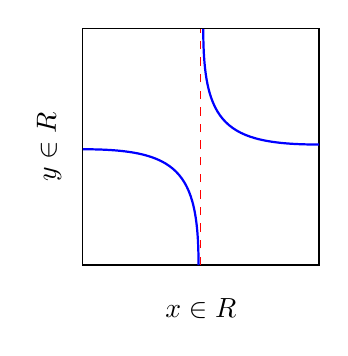
\begin{tikzpicture}[scale=0.3]
    \draw (0,0) -- (10,0) -- (10,10) -- (0,10) -- cycle;
    \draw[color=blue, thick] (0,4.9) .. controls (4,4.9) and (4.9,4) .. (4.9,0);
    \draw[color=blue, thick] (10,5.1) .. controls (6,5.1) and (5.1,6) .. (5.1,10);
    \draw[color=red, dashed] (5,0) -- (5,10);
    \node[anchor=south] at (5,-2.7) {$x \in \mathbb{R}$};
    \node[anchor=south, rotate=90] at (-0.5,5) {$y \in \mathbb{R}$};
  \end{tikzpicture}
  \hfill
  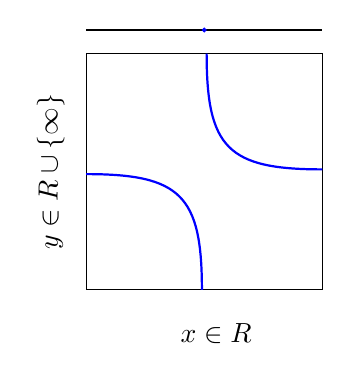
\begin{tikzpicture}[scale=0.3]
    \draw (0,0) -- (10,0) -- (10,10) -- (0,10) -- cycle;
    \draw[color=blue, thick] (0,4.9) .. controls (4,4.9) and (4.9,4) .. (4.9,0);
    \draw[color=blue, thick] (10,5.1) .. controls (6,5.1) and (5.1,6) .. (5.1,10);
    \draw (0,11) -- (10,11);
    \draw[blue,fill=blue] (5,11) circle (.5ex);
    \node[anchor=south] at (5.5,-2.7) {$x \in \mathbb{R}$};
    \node[anchor=south, rotate=90] at (-0.5,5) {$y \in \mathbb{R} \cup \{\infty\}$};
    \end{tikzpicture}
\end{frame}

\begin{filecontents*}{headdt.agda}
head : #$\forall$# {A n} → Vec A (1 + n) → A

zip : #$\forall$# {A B n} → Vec A n → Vec B n → Vec (A × B) n

take : #$\forall$# {A} m {n} → Vec A (m + n) → Vec A m
\end{filecontents*}
\begin{frame}{Safe idiom: say what you mean with dependent types}
  \inputminted{agda}{headdt.agda}
  \pause
  \bigskip
  
  (...but what properties should be reflected in the type?)
\end{frame}

%%%%%%%%%%%%%%%%%%%%%%%%%%%%%%%%%%%%%%%%%%%%%%%%%%%%%%%%%%%%%%%%%%%%%%%%
  \section{A case study in API design}   %%%%%%%%%%%%%%%%%%%%%%%%%%%%%%%
%%%%%%%%%%%%%%%%%%%%%%%%%%%%%%%%%%%%%%%%%%%%%%%%%%%%%%%%%%%%%%%%%%%%%%%%

\begin{filecontents*}{sortby.hs}
sortBy  :: (a -> a -> Ordering) -> [a]        -> [a]
mergeBy :: (a -> a -> Ordering) -> [a] -> [a] -> [a]

-- BE CAREFUL! xs and ys must already be sorted by comp!
mergeBy comp xs ys = case (xs, ys) of
    (_, []) -> xs
    ([], _) -> ys
    ((x:xs'), (y:ys')) -> case comp x y of
        LT -> x     : mergeBy comp xs' ys
        GT ->     y : mergeBy comp xs  ys'
        EQ -> x : y : mergeBy comp xs' ys'
\end{filecontents*}
\begin{frame}{A finicky API for merging and sorting}
\inputminted{haskell}{sortby.hs}    
\end{frame}

%%%%%%%%%%%%%%%%%%%%%%%%%%%%%%%%%%%%%%%%%%%%%%%%%%%%%%%%%%%%%%%%%%%%%%%%

\begin{filecontents*}{mergemay.hs}
module FancySafeMerge where
  
mergeMay :: (a -> a -> Ordering) -> [a] -> [a] -> Maybe [a]

mergeMay comp xs ys =
    if isSorted xs && isSorted ys
      then Just (mergeBy comp xs ys)
      else Nothing
      
  where     
    isSorted (z : zs@(z' : _)) =  comp z z' /= GT
                               && isSorted zs
    isSorted _ = True
\end{filecontents*}
\begin{frame}{Can we make it safe with optional types?}
\inputminted{haskell}{mergemay.hs}
\end{frame}

%%%%%%%%%%%%%%%%%%%%%%%%%%%%%%%%%%%%%%%%%%%%%%%%%%%%%%%%%%%%%%%%%%%%%%%%
\usebackgroundtemplate{%
\tikz[overlay,remember picture] \node[at=(current page.center)] {
     
\includegraphics[height=\paperheight]{angel}};
}
\begin{frame}{}\end{frame}
\usebackgroundtemplate{}

\begin{frame}{}
  \center{\Large{\textbf{Maybe more like this...}}}
\end{frame}

\usebackgroundtemplate{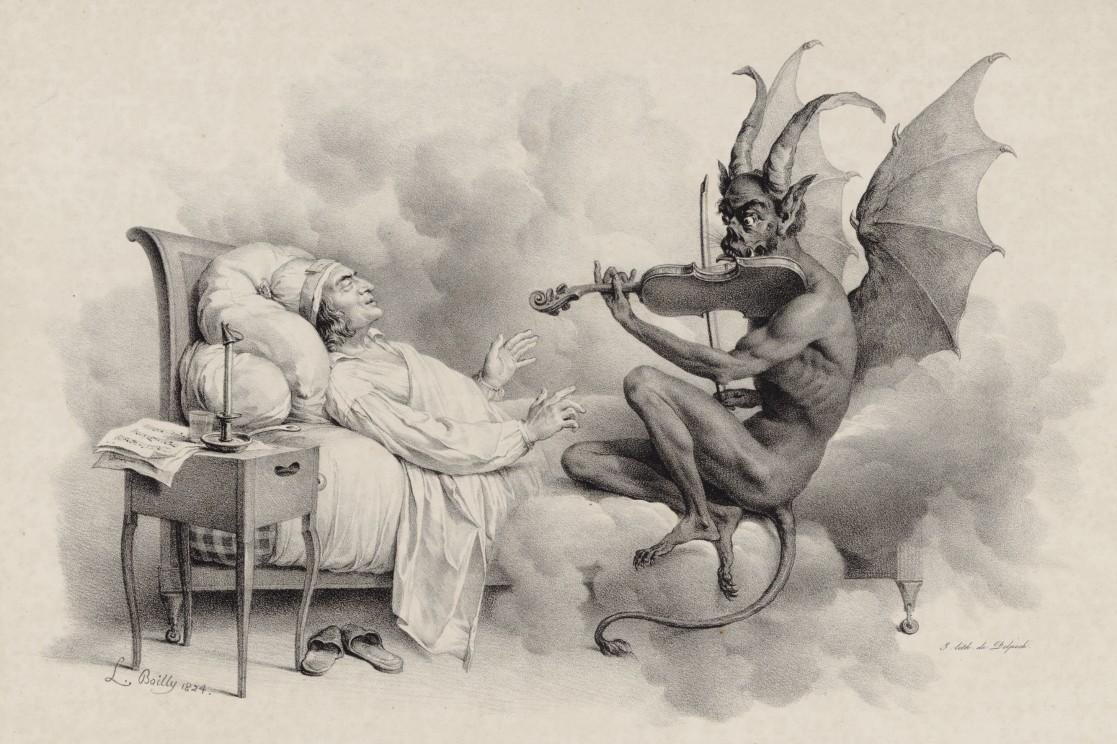
\includegraphics[width=\paperwidth,height=\paperheight]{tartinis-dream}}
\begin{frame}{}\end{frame}
\usebackgroundtemplate{}

\begin{filecontents*}{median.hs}
import FancySafeMerge

myMergeDown :: [Int] -> [Int] -> [Int]
myMergeDown xs ys =
    let comp = comparing Down
        xs' = sortBy  comp xs
        ys' = sortBy  comp ys

    in  fromJust (mergeMay comp xs' ys')
\end{filecontents*}
\begin{frame}{Leading the user into sin and vice}
\inputminted{haskell}{median.hs}

\begin{tikzpicture}[overlay, remember picture]
  \only<2>{\node[starburst, draw, minimum width=3cm, minimum height=2cm,red,text=black,opacity=0.5,fill=yellow,line width=1.5pt, above right =2.561cm and 2.76cm of current page.south west] {\footnotesize\texttt{fromJust}};}
  \end{tikzpicture}
\end{frame}

%%%%%%%%%%%%%%%%%%%%%%%%%%%%%%%%%%%%%%%%%%%%%%%%%%%%%%%%%%%%%%%%%%%%%%%%
\begin{frame}{Why is the user frustrated?}
  \begin{itemize}
    \pause\item The library API demands a precondition is met.
  \pause\item The library enforces preconditions by returning option types.
  \pause\\\bigskip

  \qquad\qquad\qquad\qquad but...
  \bigskip

  \pause
\item The user meticulously ensured that the precondition held.
  \end{itemize}
  \pause...so why are we making them check the \texttt{Nothing} case?!
\end{frame}

\begin{frame}{Frustration in the wild}
  A rough \texttt{grep} of Hackage finds over 2000 cases where \\
  {\scriptsize\texttt{lookup :: k -> Map k v -> Maybe v}} is followed by
  {\scriptsize\texttt{fromJust}}.
  \bigskip
  
  {\scriptsize\texttt{lookup}} tries to be virtuous by ensuring that the user handles the
  "missing key" case.
  \bigskip

  But what recourse is there for the gallant user who
  already proved that the key is present?
\end{frame}

%%%%%%%%%%%%%%%%%%%%%%%%%%%%%%%%%%%%%%%%%%%%%%%%%%%%%%%%%%%%%%%%%%%%%%%%
  \section{Can we do better?}   %%%%%%%%%%%%%%%%%%%%%%%%%%%%%%%%%%%%%%%%
%%%%%%%%%%%%%%%%%%%%%%%%%%%%%%%%%%%%%%%%%%%%%%%%%%%%%%%%%%%%%%%%%%%%%%%%

\begin{frame}{We want two-way communication between user and library!}
  The library author wants to tell the user ``this function can only be used when
  condition $X$ holds''.
  \bigskip
  
  The library user wants to tell the library ``I have ensured that $X$ holds, so please
  let me use the function \texttt{Maybe}-free''.
  \bigskip
  \pause
  
  \alert{Problem:} How can we reflect constraints on the function's input \emph{values} into
   the functions's \emph{type}?
\end{frame}

%%%%%%%%%%%%%%%%%%%%%%%%%%%%%%%%%%%%%%%%%%%%%%%%%%%%%%%%%%%%%%%%%%%%%%%%

\begin{filecontents*}{named-ex.hs}
module Named (name, type (~~)) where
                      -- ^ Constructor NOT exported!
import Data.Coerce

newtype a ~~ name = Named a

-- Forgetting names
instance The (a ~~ name) a where
    the = coerce :: (a ~~ name) -> a

-- Introducing names
name :: a -> (forall name. (a ~~ name) -> t) -> t
--   :: a ->  exists name. (a ~~ name)
name x cont = cont (coerce x)
\end{filecontents*}

\begin{frame}{Key idea \#1: phantom type-level names for values}
\inputminted{haskell}{named-ex.hs}
\begin{tikzpicture}[overlay, remember picture]
        \node[below right =1cm and 0.5cm of current page.north west] (A1) {};
        \node[below left  =4cm and 0.5cm of current page.north east] (A2) {};

        \node[below right =4cm and 0.5cm of current page.north west] (B1) {};
        \node[below left  =5.5cm and 0.5cm of current page.north east] (B2) {};

        \node[below right =5.8cm and 0.5cm of current page.north west] (D1) {};
        \node[below left  =8cm and 0.5cm of current page.north east] (D2) {};

        \only<2,3>{\draw[draw=none, fill=white, opacity=0.8] (A1) rectangle (A2);}
        \only<1>{\draw[draw=orange, thick] (A1) rectangle (A2); }
        \only<1,3>{\draw[draw=none, fill=white, opacity=0.8] (B1) rectangle (B2);}
        \only<2>{\draw[draw=orange, thick] (B1) rectangle (B2); }
        \only<1,2>{\draw[draw=none, fill=white, opacity=0.8] (D1) rectangle (D2);}
        \only<3>{\draw[draw=orange, thick] (D1) rectangle (D2); }
\end{tikzpicture}
\end{frame}

%%%%%%%%%%%%%%%%%%%%%%%%%%%%%%%%%%%%%%%%%%%%%%%%%%%%%%%%%%%%%%%%%%%%%%%%

\begin{filecontents*}{mergeghost.hs}
module GDP.Merge (SortedBy, mergeGDP, sortGDP) where
                  -- ^ constructor NOT exported!

-- A `SortedBy comp a` is an `a` that
-- has been sorted by `comp`.
newtype SortedBy comp a = SortedBy a

instance The (SortedBy comp a) a

-- How do we get a `SortedBy comp [a]`?
-- By sorting a list using a comparator named `comp`!
sortGDP :: ((a -> a -> Ordering) ~~ comp)
        -> [a]
        -> SortedBy comp [a]

sortGDP comp = coerce . sortBy (the comp)
\end{filecontents*}

\begin{frame}{Key idea \#2: predicates as \texttt{newtypes} + phantom types}
\inputminted{haskell}{mergeghost.hs}  
\begin{tikzpicture}[overlay, remember picture]
        \node[below right =1cm and 0.5cm of current page.north west] (A1) {};
        \node[below left  =4cm and 0.5cm of current page.north east] (A2) {};

        \node[below right =4.2cm and 0.5cm of current page.north west] (B1) {};
        \node[below left  =5.1cm and 0.5cm of current page.north east] (B2) {};

        \node[below right =5.2cm and 0.5cm of current page.north west] (D1) {};
        \node[below left  =8.8cm and 0.5cm of current page.north east] (D2) {};

        \only<2,3>{\draw[draw=none, fill=white, opacity=0.8] (A1) rectangle (A2);}
        \only<1>{\draw[draw=orange, thick] (A1) rectangle (A2); }
        \only<1,3>{\draw[draw=none, fill=white, opacity=0.8] (B1) rectangle (B2);}
        \only<2>{\draw[draw=orange, thick] (B1) rectangle (B2); }
        \only<1,2>{\draw[draw=none, fill=white, opacity=0.8] (D1) rectangle (D2);}
        \only<3>{\draw[draw=orange, thick] (D1) rectangle (D2); }
\end{tikzpicture}
\end{frame}

\begin{filecontents*}{mergeghost2.hs}
-- This type reads as:
-- "mergeGDP takes a comparator and two lists that
-- have been sorted by that same comparator.
--
-- It returns a new list that is also sorted by that
-- same comparator."

mergeGDP :: ((a -> a -> Ordering) ~~ comp)
         -> SortedBy comp [a]
         -> SortedBy comp [a]
         -> SortedBy comp [a]
         
mergeGDP comp xs ys =
    coerce (mergeBy (the comp) (the xs) (the ys))
\end{filecontents*}

\begin{frame}{How to communicate facts and requirements to the user}
\inputminted{haskell}{mergeghost2.hs}  
\end{frame}

\begin{filecontents*}{mergeghost3.hs}
import GDP.Merge

myMergeDown :: [Int] -> [Int] -> [Int]
myMergeDown xs ys =
  name (comparing Down) $ \comp ->
    let xs' = sortGDP comp xs
        ys' = sortGDP comp ys

    in      the  (mergeGDP comp xs' ys')
\end{filecontents*}
\begin{frame}{How to communicate due-dilligence back to the library}
  \inputminted{haskell}{median.hs}  
\end{frame}

\begin{frame}{How to communicate due-dilligence back to the library}
  \inputminted{haskell}{mergeghost3.hs}  
\end{frame}

\begin{frame}{Key idea \#3: ghosts disappear on compilation}
  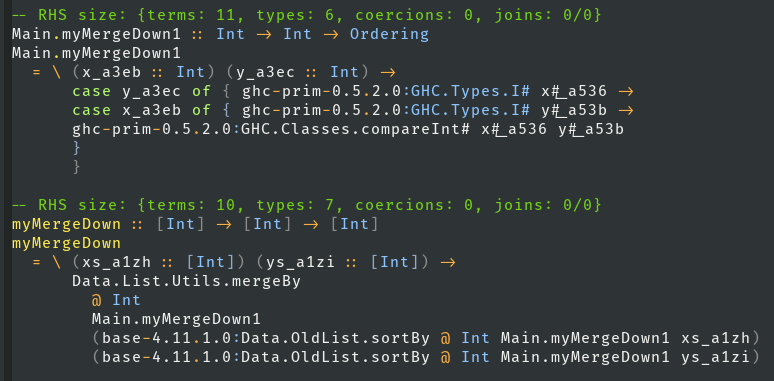
\includegraphics[width=0.8\paperwidth]{simpl}
\end{frame}

%%%%%%%%%%%%%%%%%%%%%%%%%%%%%%%%%%%%%%%%%%%%%%%%%%%%%%%%%%%%%%%%%%%%%%%%
  \section{Ghosts of Departed Proofs}   %%%%%%%%%%%%%%%%%%%%%%%%%%%%%%%%
%%%%%%%%%%%%%%%%%%%%%%%%%%%%%%%%%%%%%%%%%%%%%%%%%%%%%%%%%%%%%%%%%%%%%%%%

  \usebackgroundtemplate{%
\tikz[overlay,remember picture] \node[at=(current page.center)] {
   
\includegraphics[height=\paperheight]{limit}};
}
\begin{frame}{}\end{frame}
\usebackgroundtemplate{}
%%%%%%%%%%%%%%%%%%%%%%%%%%%%%%%%%%%%%%%%%%%%%%%%%%%%%%%%%%%%%%%%%%%%%%%%

\begin{frame}{Some lingering questions}

  \begin{itemize}
  \item How do we decide which properties get \texttt{newtype} wrappers?
  \bigskip

\item How do we handle properties involving multiple values?
  \bigskip
  
\item How do we know that we have given the user enough information to complete their proofs?
  \end{itemize}
\end{frame}

%%%%%%%%%%%%%%%%%%%%%%%%%%%%%%%%%%%%%%%%%%%%%%%%%%%%%%%%%%%%%%%%%%%%%%%%
\begin{filecontents*}{gdp-ex.hs}
module GDP (Proof, axiom, {- etc -}) where

data Proof p = QED

axiom :: String -> Proof p
axiom reason = QED

newtype a ::: p = WithContext a
instance The (a ::: p) a

toContext   :: Proof p -> a -> (a ::: p)
fromContext :: (a ::: p)    -> Proof p

class Fact p

note   :: Proof p -> (Fact p => t) -> t
recall :: (Fact p => t) -> Proof p
\end{filecontents*}
\begin{filecontents*}{gdp-comb.hs}
-- module GDP, continued:
data p || q
data p && q
data x == y

orIntroL :: Proof p -> Proof (p || q)

orElim :: (Proof p        -> Proof r)
       -> (Proof q        -> Proof r)
       -> (Proof (p || q) -> Proof r)
       
andIntro :: Proof p -> Proof q -> Proof (p && q)

refl :: Proof (x == x)

-- ...and many, many more
\end{filecontents*}

\begin{frame}{Key idea \#4: ghostly proofs}
\inputminted{haskell}{gdp-ex.hs}
\begin{tikzpicture}[overlay, remember picture]
        \node[below right =1cm and 0.5cm of current page.north west] (A1) {};
        \node[below left  =4.1cm and 0.5cm of current page.north east] (A2) {};

        \node[below right =4.1cm and 0.5cm of current page.north west] (B1) {};
        \node[below left  =6.9cm and 0.5cm of current page.north east] (B2) {};

        \node[below right =6.9cm and 0.5cm of current page.north west] (C1) {};
        \node[below left  =9.2cm and 0.5cm of current page.north east] (C2) {};

        \only<2,3>{\draw[draw=none, fill=white, opacity=0.8] (A1) rectangle (A2);}
        \only<1>{\draw[draw=orange, thick] (A1) rectangle (A2); }
        \only<1,3>{\draw[draw=none, fill=white, opacity=0.8] (B1) rectangle (B2);}
        \only<2>{\draw[draw=orange, thick] (B1) rectangle (B2); }
        \only<1,2>{\draw[draw=none, fill=white, opacity=0.8] (C1) rectangle (C2);}
        \only<3>{\draw[draw=orange, thick] (C1) rectangle (C2); }
\end{tikzpicture}
\end{frame}

\begin{frame}{Proof combinators}
\inputminted{haskell}{gdp-comb.hs}
\end{frame}

%%%%%%%%%%%%%%%%%%%%%%%%%%%%%%%%%%%%%%%%%%%%%%%%%%%%%%%%%%%%%%%%%%%%%%%%
\begin{filecontents*}{listshape.hs}
data IsNil  xs
data IsCons xs  

pattern Nil  :: () => Fact (IsNil  xs) => ([a] ~~ xs)
pattern Cons :: () => Fact (IsCons xs) => ([a] ~~ xs)

head :: Fact (IsCons xs) => ([a] ~~ xs) ->  a
head xs = Prelude.head (the xs)

tail :: Fact (IsCons xs) => ([a] ~~ xs) -> [a]
tail xs = Prelude.tail (the xs)
\end{filecontents*}

\begin{filecontents*}{safehead.hs}
newtype Reverse xs = Reverse Defn

reverse :: ([a] ~~ xs) -> ([a] ~~ Reverse xs)
reverse xs = defn (Prelude.reverse (the xs))

rev'rev  :: Proof (xs == Reverse (Reverse xs))
rev'rev = axiom "reversing twice is identity"

rev'cons ::
  Proof (IsCons xs) -> Proof (IsCons (Reverse xs))
rev'cons _ = axiom "reverse preserves cons-ness"
\end{filecontents*}

\begin{frame}{Ghosts of list shapes}
\inputminted{haskell}{listshape.hs}
\begin{tikzpicture}[overlay, remember picture]
        \node[below right =1.9cm and 0.5cm of current page.north west] (A1) {};
        \node[below left  =4.5cm and 0.5cm of current page.north east] (A2) {};

        \node[below right =4.5cm and 0.5cm of current page.north west] (B1) {};
        \node[below left  =7.5cm and 0.5cm of current page.north east] (B2) {};

        \only<2>{\draw[draw=none, fill=white, opacity=0.8] (A1) rectangle (A2);}
        \only<1>{\draw[draw=orange, thick] (A1) rectangle (A2); }
        \only<1>{\draw[draw=none, fill=white, opacity=0.8] (B1) rectangle (B2);}
        \only<2>{\draw[draw=orange, thick] (B1) rectangle (B2); }
\end{tikzpicture}
\end{frame}

\begin{frame}{Library-provided lemmas}
\inputminted{haskell}{safehead.hs}
\begin{tikzpicture}[overlay, remember picture]
        \node[below right =1.9cm and 0.5cm of current page.north west] (A1) {};
        \node[below left  =4cm and 0.5cm of current page.north east] (A2) {};

        \node[below right =4cm and 0.5cm of current page.north west] (B1) {};
        \node[below left  =7.5cm and 0.5cm of current page.north east] (B2) {};

        \only<2>{\draw[draw=none, fill=white, opacity=0.8] (A1) rectangle (A2);}
        \only<1>{\draw[draw=orange, thick] (A1) rectangle (A2); }
        \only<1>{\draw[draw=none, fill=white, opacity=0.8] (B1) rectangle (B2);}
        \only<2>{\draw[draw=orange, thick] (B1) rectangle (B2); }
\end{tikzpicture}
\end{frame}

\begin{filecontents*}{uselist.hs}
main :: IO ()
main = do
  args <- getArgs
  name args $ \args -> case args of
    Nil  -> putStrLn "No arguments!"
    Cons -> noting rev'cons args $ do
      print (head args)
      print (head (reverse args))
\end{filecontents*}
\begin{filecontents*}{uselist-wrong.hs}
main :: IO ()
main = do
  args <- getArgs
  name args $ \args -> case args of
    Nil  -> putStrLn "No arguments!"
    Cons -> do
      print (head args)
      print (head (reverse args))
\end{filecontents*}
\begin{frame}{Using the safe list API}
  \inputminted{haskell}{uselist-wrong.hs}
\only<2>{\begin{tikzpicture}[overlay,remember picture] \node[below =1.8cm of current page.center] {
    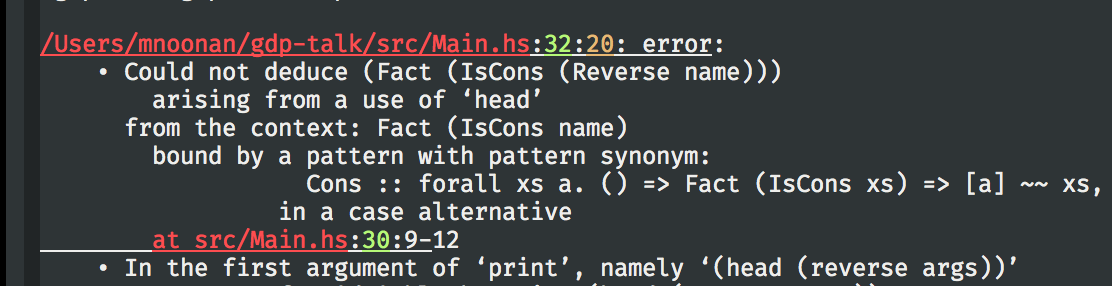
\includegraphics[height=2.7cm]{error}};
  \end{tikzpicture}}
\end{frame}
\begin{frame}{Using the safe list API}
  \inputminted{haskell}{uselist.hs}
\end{frame}

%%%%%%%%%%%%%%%%%%%%%%%%%%%%%%%%%%%%%%%%%%%%%%%%%%%%%%%%%%%%%%%%%%%%%%%%
  \section{Summary}   %%%%%%%%%%%%%%%%%%%%%%%%%%%%%%%%%%%%%%%%%%%%%%%%%%
%%%%%%%%%%%%%%%%%%%%%%%%%%%%%%%%%%%%%%%%%%%%%%%%%%%%%%%%%%%%%%%%%%%%%%%%
\begin{frame}{API design with Ghosts of Departed Proofs}
  \begin{itemize}
  \item{Use \alert{existentially-quantified names} to discuss values at the type level.}
  \bigskip
  \item{Avoid boolean blindness by \alert{returning proofs to the user}.}
  \bigskip
  \item{Avoid runtime overhead by putting \alert{proofs in phantom types}.}
  \bigskip
  \item{Give the user \alert{combinators for constructing proofs}.}
  \end{itemize}

\end{frame}

%%%%%%%%%%%%%%%%%%%%%%%%%%%%%%%%%%%%%%%%%%%%%%%%%%%%%%%%%%%%%%%%%%%%%%%%

\begin{frame}{Try it out!}
  \begin{itemize}
  \item{The \texttt{gdp} library is on Hackage and Stackage
    \url{http://hackage.haskell.org/package/gdp}\medskip
  }
  \item{The paper's repo has smaller examples that are easy to play with
    in \texttt{ghci} (see the \texttt{gdp-demo} subdirectory)
    \url{https://github.com/matt-noonan/gdp-paper}\medskip}
  \item{\texttt{chessai} implemented the ``\texttt{ST}-with-sharing'' code
    in the \texttt{st2} library (also on Hackage) \url{https://github.com/chessai/st2}}
  \end{itemize}
  \medskip
  \Large{Thank you for your time!}
\end{frame}

\begin{filecontents*}{jmap.hs}
-- Ghosts of departed key sets
newtype JMap keys k v = JMap (Map k v)
newtype k #$\in$# keys      = Key k

-- Key search, avoiding boolean blindness
member :: Ord k => k -> JMap keys k v -> Maybe (k #$\in$# keys)
member k m = if Map.member k (the m)
               then Just (coerce k)
               else Nothing
               
-- Maybe-free lookup
lookup :: Ord k => (k #$\in$# keys) -> JMap keys k v -> v
lookup k m = fromJust (Map.lookup (the k) (the m))

-- A safe adjacency-list type for directed graphs
type Digraph k v = JMap keys k [k #$\in$# keys]
\end{filecontents*}

\section{Additional examples}

\begin{frame}{Maybe-free lookup in maps}
\inputminted{haskell}{jmap.hs}
\begin{tikzpicture}[overlay, remember picture]
        \node[below right =1cm and 0.5cm of current page.north west] (A1) {};
        \node[below left  =2.7cm and 0.5cm of current page.north east] (A2) {};

        \node[below right =2.7cm and 0.5cm of current page.north west] (B1) {};
        \node[below left  =5.5cm and 0.5cm of current page.north east] (B2) {};

        \node[below right =5.5cm and 0.5cm of current page.north west] (C1) {};
        \node[below left  =7.5cm and 0.5cm of current page.north east] (C2) {};

        \node[below right =7.5cm and 0.5cm of current page.north west] (D1) {};
        \node[below left  =8.7cm and 0.5cm of current page.north east] (D2) {};

        \only<2,3,4>{\draw[draw=none, fill=white, opacity=0.8] (A1) rectangle (A2);}
        \only<1>{\draw[draw=orange, thick] (A1) rectangle (A2); }
        \only<1,3,4>{\draw[draw=none, fill=white, opacity=0.8] (B1) rectangle (B2);}
        \only<2>{\draw[draw=orange, thick] (B1) rectangle (B2); }
        \only<1,2,4>{\draw[draw=none, fill=white, opacity=0.8] (C1) rectangle (C2);}
        \only<3>{\draw[draw=orange, thick] (C1) rectangle (C2); }
        \only<1,2,3>{\draw[draw=none, fill=white, opacity=0.8] (D1) rectangle (D2);}
        \only<4>{\draw[draw=orange, thick] (D1) rectangle (D2); }
\end{tikzpicture}
\end{frame}


\begin{filecontents*}{hashes.hs}
newtype HashOf x = HashOf Defn

realHash :: Serializable a =>  a       ->  Hash
hash     :: Serializable a => (a ~~ x) -> (Hash ~~ HashOf x)

hash x = defn (realHash (serialize $ the x))

-- A type for objects along with their hash.
data ThingWithHash a = forall x. ThingWithHash
  { _thing :: a    ~~ x
  , _hash  :: Hash ~~ HashOf x }

-- Use it like this:
hashIt :: Serializable a => a -> ThingWithHash a
hashIt x = name x $ \x' ->
  ThingWithHash { _thing = x', _hash = hash x' }
                          
    
\end{filecontents*}

\begin{frame}{Hashed data structures}
\inputminted{haskell}{hashes.hs}
\end{frame}

\begin{filecontents*}{st2.hs}
-- Running an ST computation with shared regions
runSt2  ::
  STRef (forall mine yours. ST (mine #$\cap$# yours) a) -> a

inMine  :: ST mine  a -> ST (mine #$\cap$# yours) a
inYours :: ST yours a -> ST (mine #$\cap$# yours) a

-- Sharing an STRef we own
share  :: STRef mine a -> ST mine (STRef (mine #$\cap$# yours) a)

-- Using an STRef that was shared with us
use    :: STRef (mine #$\cap$# yours) a -> STRef mine a

-- Algebraic lemmas
symm   :: STRef (mine #$\cap$# yours) a -> STRef (yours #$\cap$# mine) a

\end{filecontents*}

\usebackgroundtemplate{
\includegraphics[width=\paperwidth,height=\paperheight]{sharing}}
\begin{frame}{}\end{frame}

\usebackgroundtemplate{}
\begin{frame}{The ST monad, with shared memory regions}
  \inputminted{haskell}{st2.hs}
\end{frame}


\end{document}


